% author: Man Cao, Lilong Jiang
\documentclass{article}
\usepackage[letterpaper]{geometry} \usepackage[utf8]{inputenc}
\usepackage[T1]{fontenc}
\usepackage{amsmath}
\usepackage{hyperref}
\usepackage{relsize}
\usepackage{graphicx}

\newcommand{\code}[1]{\textsf{\smaller\verb~#1~}}

\begin{document}

\title{CSE5243 Assignment 2}
\author{Man Cao(cao.235), Lilong Jiang(jiang.573)}
\maketitle

\section{Work Separation}
Lilong mainly worked on K-nearest neighbor classifier. Man mainly worked on
Naive Bayesian classifier. In fact there were a lot of overlapping during the
work, we exchanged various ideas and wrote the this report together.
\section{Input}
After eliminating documents without topics, 11367 documents are left.\\
We also made some slight changes to the preprocessor from project 1, including
removing words that contains less than 3 letters, and short words with
punctuations (such as ``'s'').
The input file has the following format:
\begin{verbatim}
{'NEWID':<value>, 'TOPICS':[value1, value2, ...], 'PLACES':[value1, value2, ...]}
{<term1>:<value1>, <term1>:<value2>, ...}
\end{verbatim}
Note that each document corresponds to two lines: the first line contains the
metadata of the document, the second line is the frequency vector.

\section{Algorithms and Methodology}
We have implemented K-nearest neighbor (KNN) and Naive Bayesian (Bayes) classification algorithms.
We perform a 5-fold cross validation. The final results are averaged across 5
rounds.

In order to predict multiple topics for a given document, we set a parameter M
to limit the maximum number of topics for the document.
For each classifier, the top--M topics with the greatest \emph{likelihood} are
considered as the topics for the document. E.g. if M = 1, each document will
have one predicted topic; if M = 2, each document will have two predicted topics.
For KNN, the likelihood is the count of documents for each topic in the top-K most similar documents;
for Bayes, it is the probability of the each topic.

When measuring precision for document multiple topics, if one of the predicted
topics is a correct topic, we just consider the classification is correct.

\subsection{K-nearest neighbor}
\subsubsection{Build the model}
K is selected according to the following equation:
\begin{align*}K = \sqrt[2]{N}\end{align*}
where $N$ is the number of documents in the training dataset.
\subsubsection{Test the model}
For every test document, we computes the cosine similarity between the test document and all the other documents.
\subsubsection{Implementation Details}
A min-heap is used to maintain the top-K nearest neighbor. Everytime a new similarity is computed, we will compare it with the minimum value in the min-heap, if the new similarity is greater than the minimum similarity in the heap, we will update the min-heap. In this way, we can achieve $Nlog K$ time complexity.
\subsection{Naive Bayesian}
\subsubsection{Build the model}
The topics in the document are used to build the classes. The documents with multiple topics are assigned to the each respective class, so they are counted multiple times. 

\subsubsection{Test the model}
The probability of document D in class $C_i$ $P(C_i|D)$ is calculated as
follows:
\begin{align*}
P(C_i|D) = \frac{P(D|C_i) \times P(C_i)}{P(D)}
	 = \frac{P(W_1|C_i) \times P(W_2|C_i) \times ... \times P(W_n|C_i) \times P(C_i)}{P(D)}				
\end{align*}
where $C_i$ denotes the i-th class, D denotes the test document. $P(C_i)$ is computed as the number of documents in class $C_i$ over the number of documents in the training dataset. $P(W_j|C_i)$ is computed as the number of documents containing word $W_j$ over the number of documents in class $C_i$.

\subsection{Implementation Details}
\begin{itemize}
\item M-estimate of Conditional Probability\\
In order to handle the case that the training dataset do not cover all the words in the document, we use m-estimate approach to estimating the conditional probability, which is shown as the following:
\begin{align*}
P(W_j|C_i) = \frac{n_c + m \times p}{n + m}
\end{align*}
where $n_c$ is the number of documents from class $C_i$ that contain word $W_j$, n is the number of documents in $C_i$, m is the size of the training dataset, p is the prior probability of word $W_j$ which is calculated as the number of documents containing the word $W_j$ in the training dataset over the size of the training dataset. For a word not occurring in the training dataset, we assume p is 0.01 over the size of the training set.
\end{itemize}

We have tried an alternative way to compute $P(W_j|C_i)$, which takes the frequency of each word into account. However, preliminary results show that its precision is almost the same as the standard approach, so we did not further investigate this approach. 
\section{Evaluation}
Our program is run on the stdlinux.
\subsection{Precision}
Precision is the fraction of retrieved instances that are relevant. Results are shown in Figure~\ref{Fig:prec}.\\
The average precision of 5-fold cross validation is 79.7\% for K nearest neighbor method with M = 1 while 89.8\% with M = 2.\\
The average precision of 5-fold cross validation is 74.1\% for naive bayesian classifier with M = 1, while 81.6\% with M = 2. 
\begin{figure}
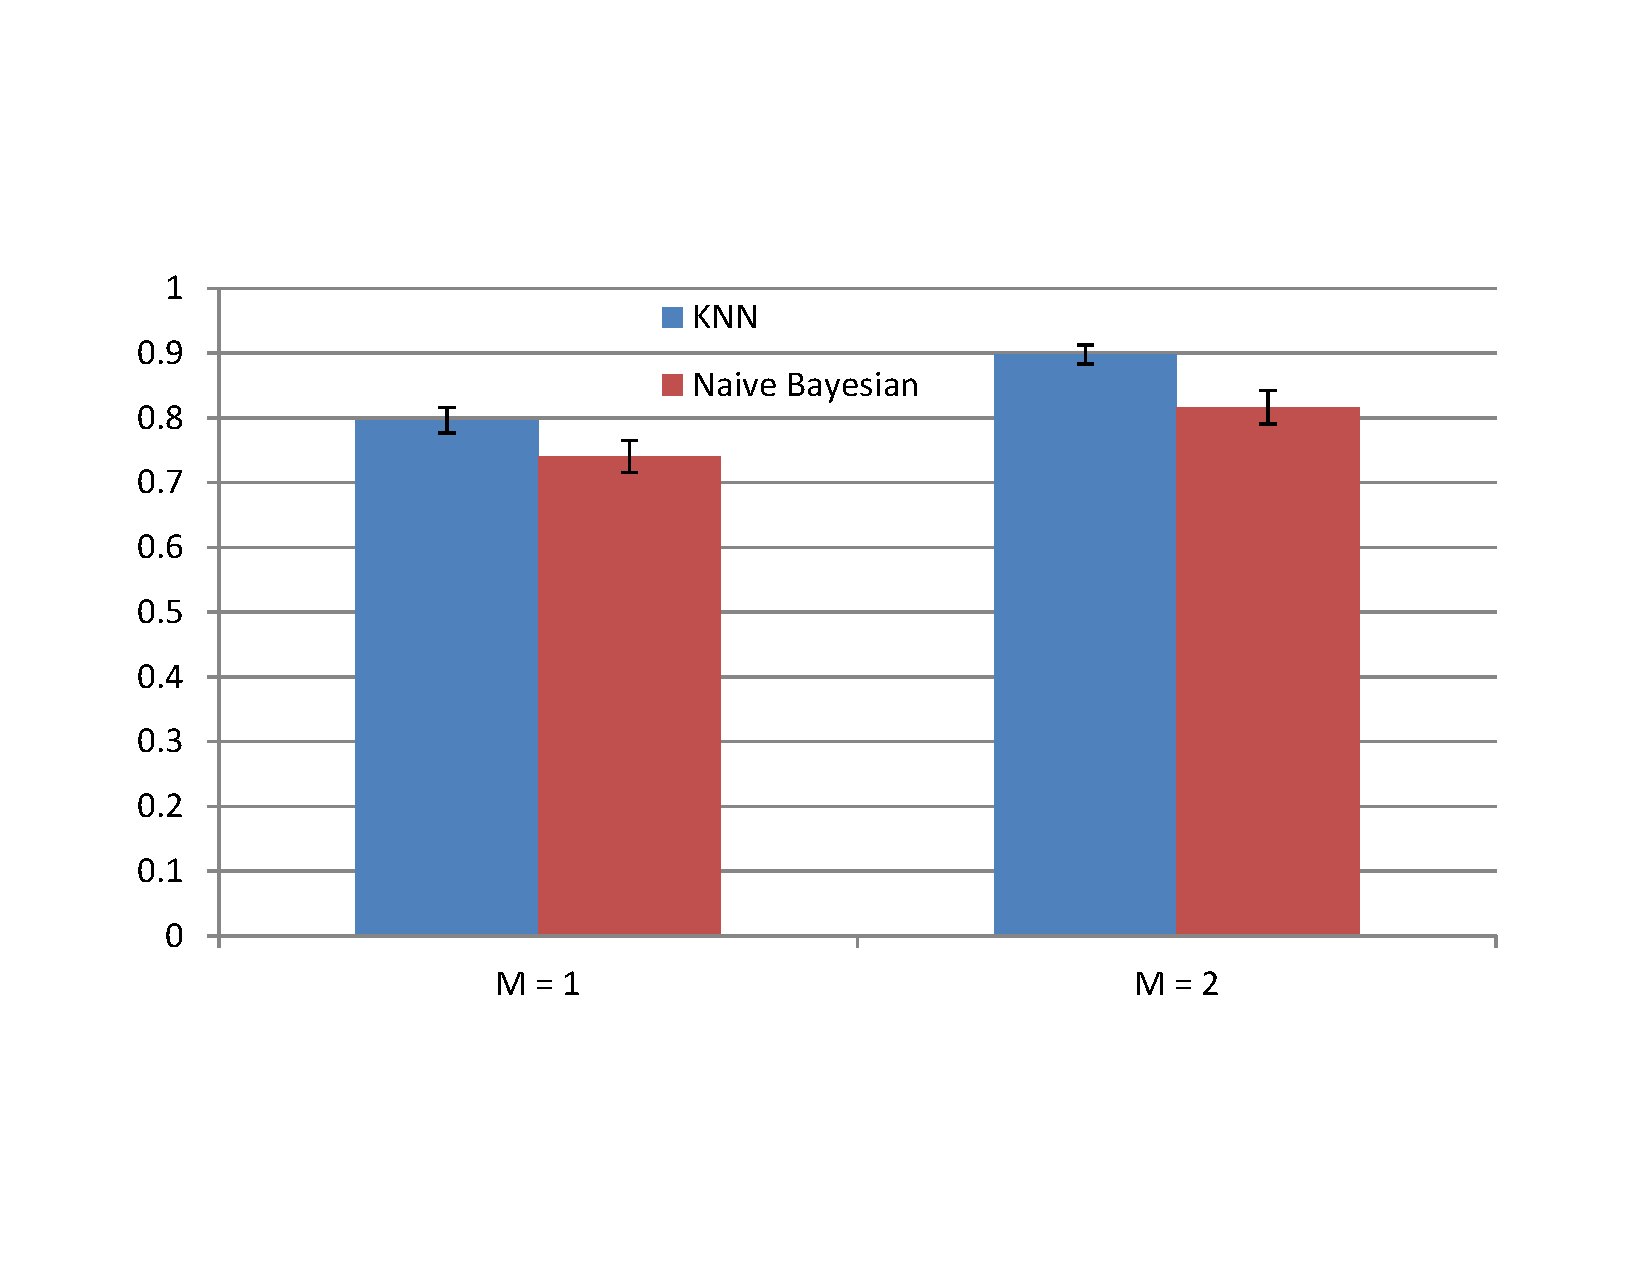
\includegraphics[width=1.0\textwidth]{Precision}
\caption{The average precision in percentage for each classifier over 5-fold cross validation, for two M values. }
\label{Fig:prec}
\end{figure}

\subsection{Training Time}
For KNN, the training time mainly means the time for selecting K. It is negligible in our algorithm since K is computed as a root square of the number of documents in the training dataset.\\
For naive baysian classifier, the time for build the classes from 9094 documents is 0.39s on average.
\subsection{Test Time}
We calculate the time for classifying one document. Results are shown in Figure~\ref{Fig:perf}. The time for KNN is 0.19s on average while 0.006s for naive bayesian classifier.


\begin{figure}
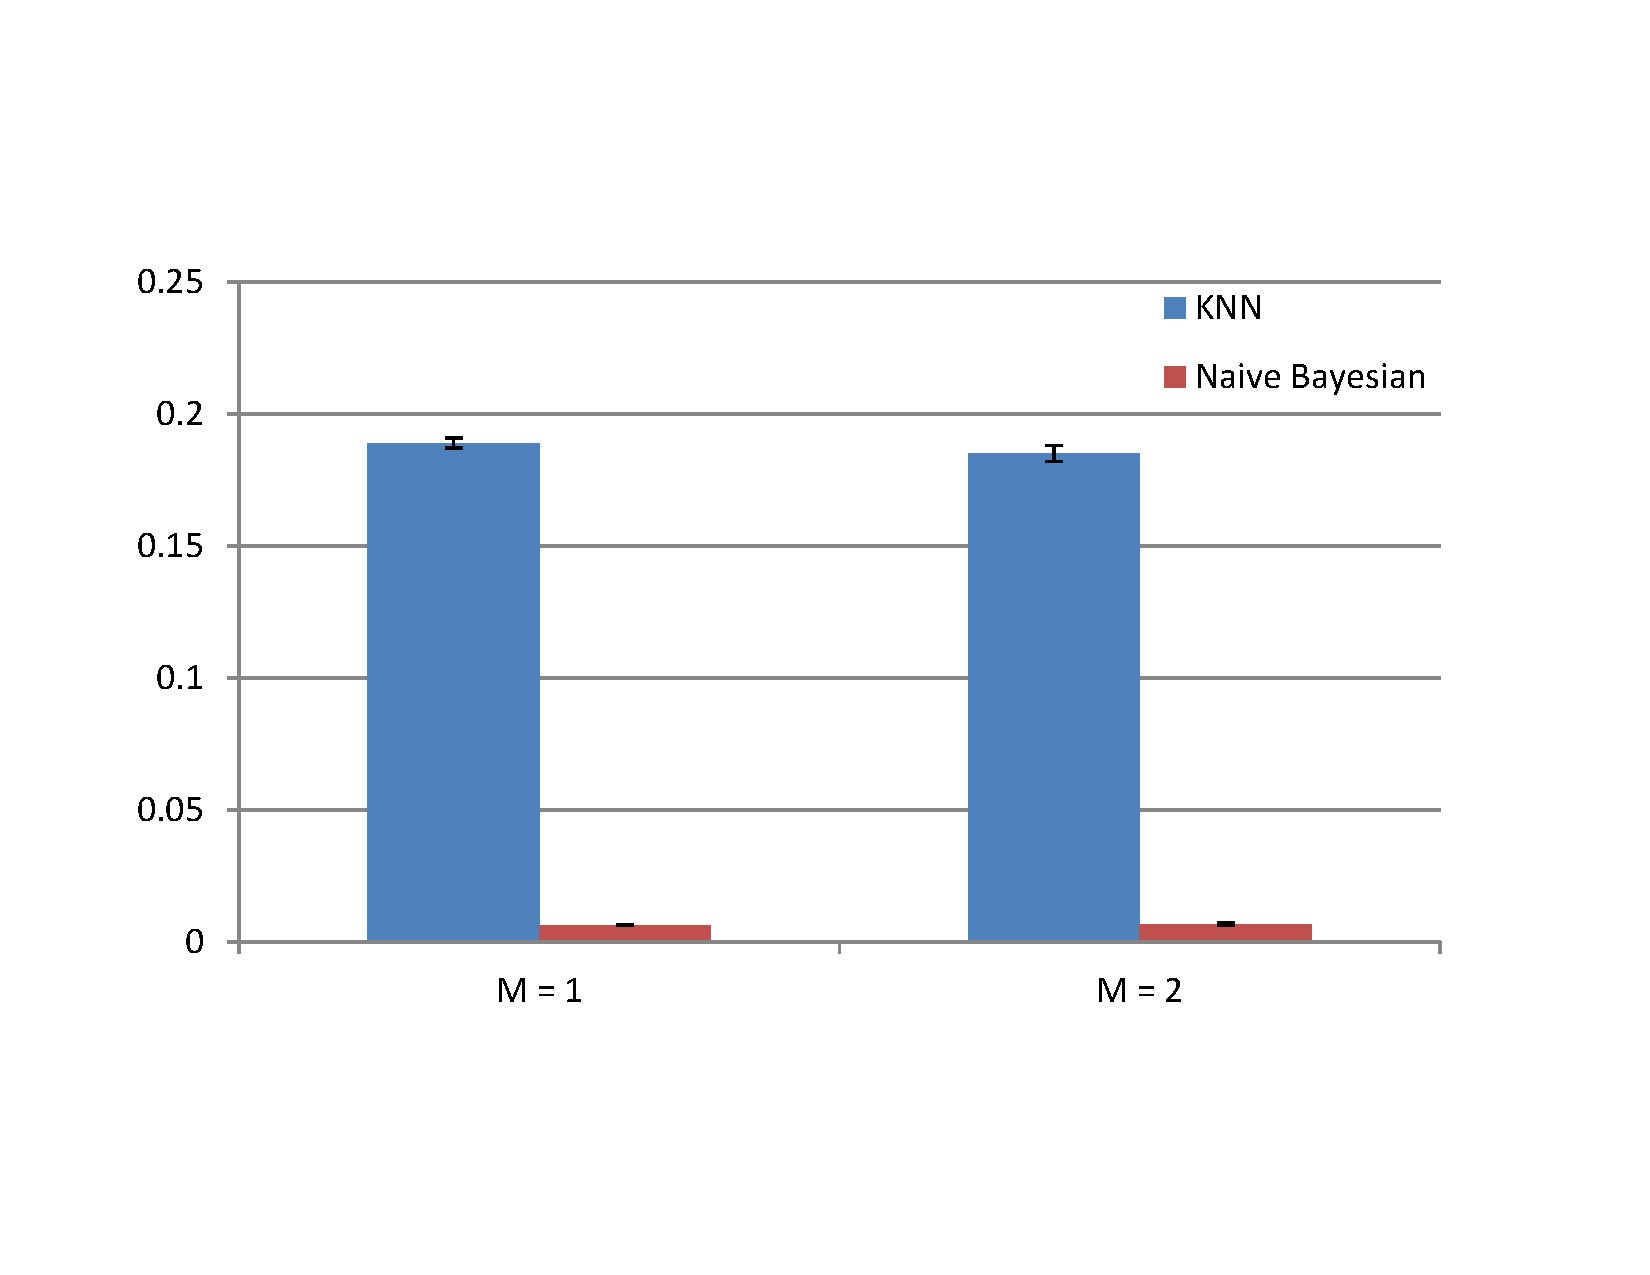
\includegraphics[width=1.0\textwidth]{TestTime}
\caption{The average test time in second for each classifier over 5-fold cross validation, for two M values.}
\label{Fig:perf}
\end{figure}
\end{document}

